\documentclass[a4paper,12pt]{article} % тип документа

% Поля страниц
\usepackage[left=2.5cm,right=2.5cm,
    top=2cm,bottom=2cm,bindingoffset=0cm]{geometry}
    
%Пакет дял таблиц   
\usepackage{multirow} 
    
%Отступ после заголовка    
\usepackage{indentfirst}


% Рисунки
\usepackage{floatrow,graphicx,calc}
\usepackage{wrapfig}

%%% Работа с картинками
\usepackage{graphicx}  % Для вставки рисунков
\graphicspath{{images/}{images2/}}  % папки с картинками
\setlength\fboxsep{3pt} % Отступ рамки \fbox{} от рисунка
\setlength\fboxrule{1pt} % Толщина линий рамки \fbox{}
\usepackage{wrapfig} % Обтекание рисунков и таблиц текстом

% Создаёем новый разделитель
\DeclareFloatSeparators{mysep}{\hspace{1cm}}

% Ссылки?
\usepackage{hyperref}
\usepackage[rgb]{xcolor}
\hypersetup{				% Гиперссылки
    colorlinks=true,       	% false: ссылки в рамках
	urlcolor=blue          % на URL
}


%  Русский язык
\usepackage[T2A]{fontenc}			% кодировка
\usepackage[utf8]{inputenc}			% кодировка исходного текста
\usepackage[english,russian]{babel}	% локализация и переносы




% Математика
\usepackage{amsmath,amsfonts,amssymb,amsthm,mathtools}

%%% Дополнительная работа с математикой
\usepackage{amsmath,amsfonts,amssymb,amsthm,mathtools} % AMS
\usepackage{icomma} % "Умная" запятая: $0,2$ --- число, $0, 2$ --- перечисление


% Что-то 
\usepackage{wasysym}


\begin{document}
\begin{center}
	\footnotesize{ФЕДЕРАЛЬНОЕ ГОСУДАРСТВЕННОЕ АВТОНОМНОЕ ОБРАЗОВАТЕЛЬНОЕ 			УЧРЕЖДЕНИЕ ВЫСШЕГО ОБРАЗОВАНИЯ}\\
	\footnotesize{МОСКОВСКИЙ ФИЗИКО-ТЕХНИЧЕСКИЙ ИНСТИТУТ\\(НАЦИОНАЛЬНЫЙ 			ИССЛЕДОВАТЕЛЬСКИЙ УНИВЕРСИТЕТ)}\\
	\hfill \break
	\hfill \break
	\hfill \break
	\hfill \break
\end{center}

  \hfill \break
\hfill \break
\hfill \break
\hfill \break
\hfill \break
\hfill \break
\hfill \break
\hfill \break



\begin{center}   
    \hfill \break
	\hfill \break
	\hfill \break
	\large{Лабораторная работа № 3.2.8\\ \hfill \break\Large{Релаксационные колебания}}\\
	\hfill \break
	\hfill \break
	\hfill \break
	\hfill \break
	\begin{flushright}
		Сирый Р.А.\\
		Б02-206
	\end{flushright}
	\hfill \break
	\hfill \break
	\hfill \break
\end{center}
\hfill \break
\hfill \break
\hfill \break
\hfill \break
\begin{center}
	Долгопрудный, 2023 г.
\end{center}
\thispagestyle{empty}

\newpage

\textbf{Цель работы:} изучение вольтамперной характеристики нормального тлеющего заряда; исследование релаксационного генератора на стабилитроне.

\textbf{В работе используются:} стабилитрон СГ-2 (газонаполненный диод) на монтажной панели, магазин ёмкостей, магазин сопротивлений, источник питания, амперметр, вольтметр, осциллограф.

\section{Теоретические сведения}

 Колебательные системы, как правило, имеют два накопителя, между которыми происходит перекачка энергии. В контуре, содержащем конденсатор и катушку индуктивности, электрическая энергия переходит в магнитную и обратно; при колебаниях маятника потенциальная энергия поля тяжести переходит в кинетическую энергию движущейся массы и т.д. 

\begin{wrapfigure}{r}{0.3\textwidth} 
\begin{center}
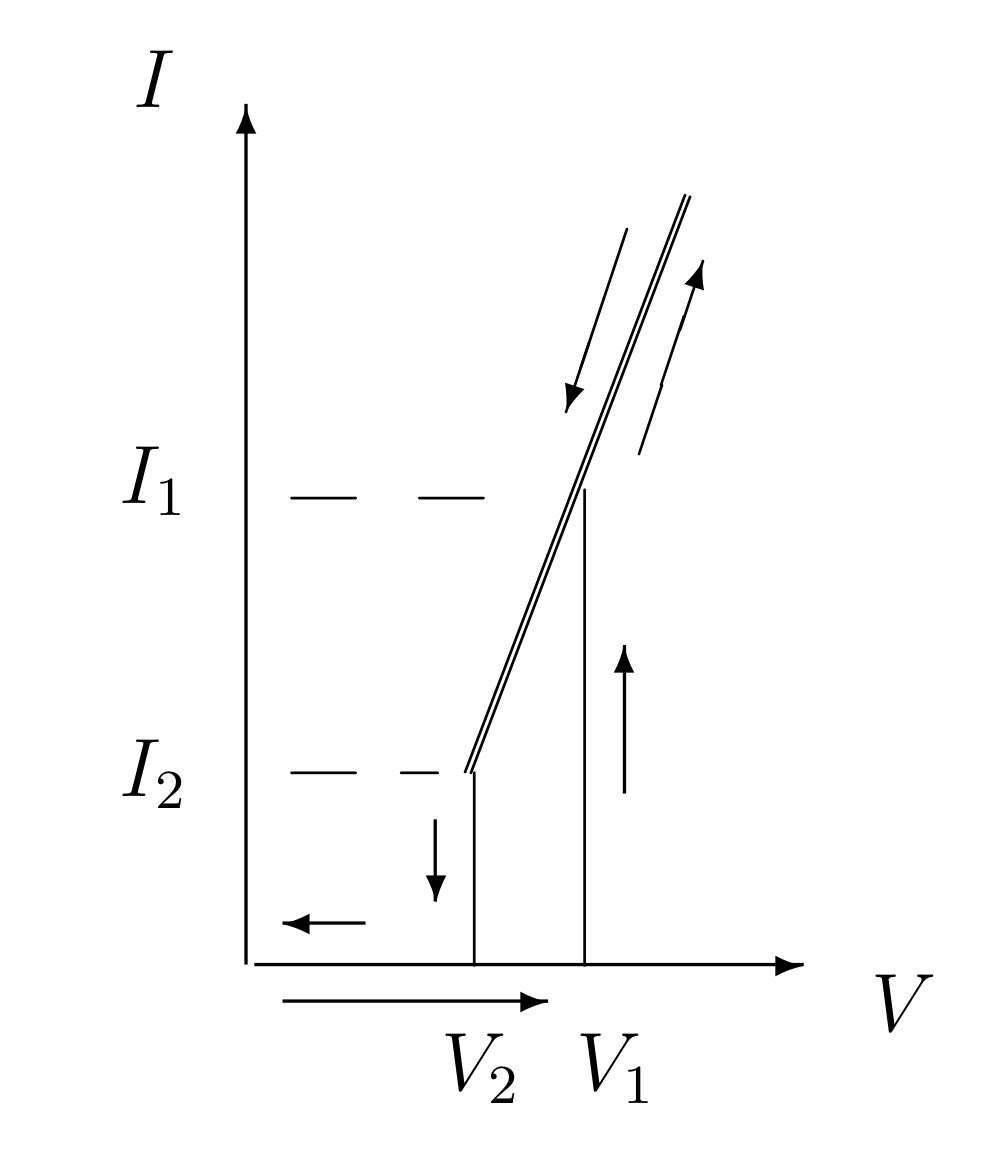
\includegraphics[width=1\textwidth]{graph.jpg} 
\caption{\centering{Вольтамперная характеристика стабилитрона с последовательно включенным резистором}}
\end{center}
\end{wrapfigure}

Встречаются, однако, колебательные системы, содержащие всего один накопитель энергии. Рассмотрим в качестве примера электрическую цепь, содержащую конденсатор и сопротивление без самоиндукции. Разряд конденсатора через сопротивление представляет собой апериодический процесс. Разряду, однако, можно придать периодический характер, возобновляя заряд конденсатора через постоянные промежутки времени. Колебания в этом случае являются совокупностью двух апериодических процессов - процесса зарядки конденсатора и процесса его разрядки. Такие колебания называются релаксационними.\\
В нашей установке роль ключа, обеспечивающего последовательно попеременную зарядку и разрядку конденсатора, играет газоразрядный диод. Зависимость тока от напряжения для газоразрядной лампы не подчиняется закону Ома и характеризуется рядом особенностей (рис. 1). При малых напряжениях лампа не пропускает тока вовсе (не горит). Ток в лампе возникает только в том случае, если разность потенциалов на её электродах достигает напряжения зажигания $V_{1} .$ При этом, тлеюиций разряд. При дальнейшем незначительном увеличении напряжения сила тока заметно возрастает по закону, близкому к линейному. 
Если начать уменьшать напряжение на горящей лампе, то при напряжении, равном $V_{1},$ лампа ещё не гаснет, и сила тока продолжает уменьшаться. Лампа перестанет пропускать ток лишь при напряжении гашения $V_{2},$ которое обычно существенно меньше $V_{1}$. Сила тока при этом скачком падает от значения $I_{2}\left(I_{2}<I_{1}\right)$ до нуля. Характеристика, изображённая на рис. 1, несколько идеализирована. $\mathrm{Y}$ реальной лампы зависимость $I(V)$ не вполне линейна. При $V>V_{1}$ графики
соответствующие возрастанию и убыванию напряжения, не всегда совпадают. Эти отличия, впрочем, носят второстепенный характер и для нашей задачи несущественны.


\begin{wrapfigure}{r}{0.3\textwidth} 
\begin{center}
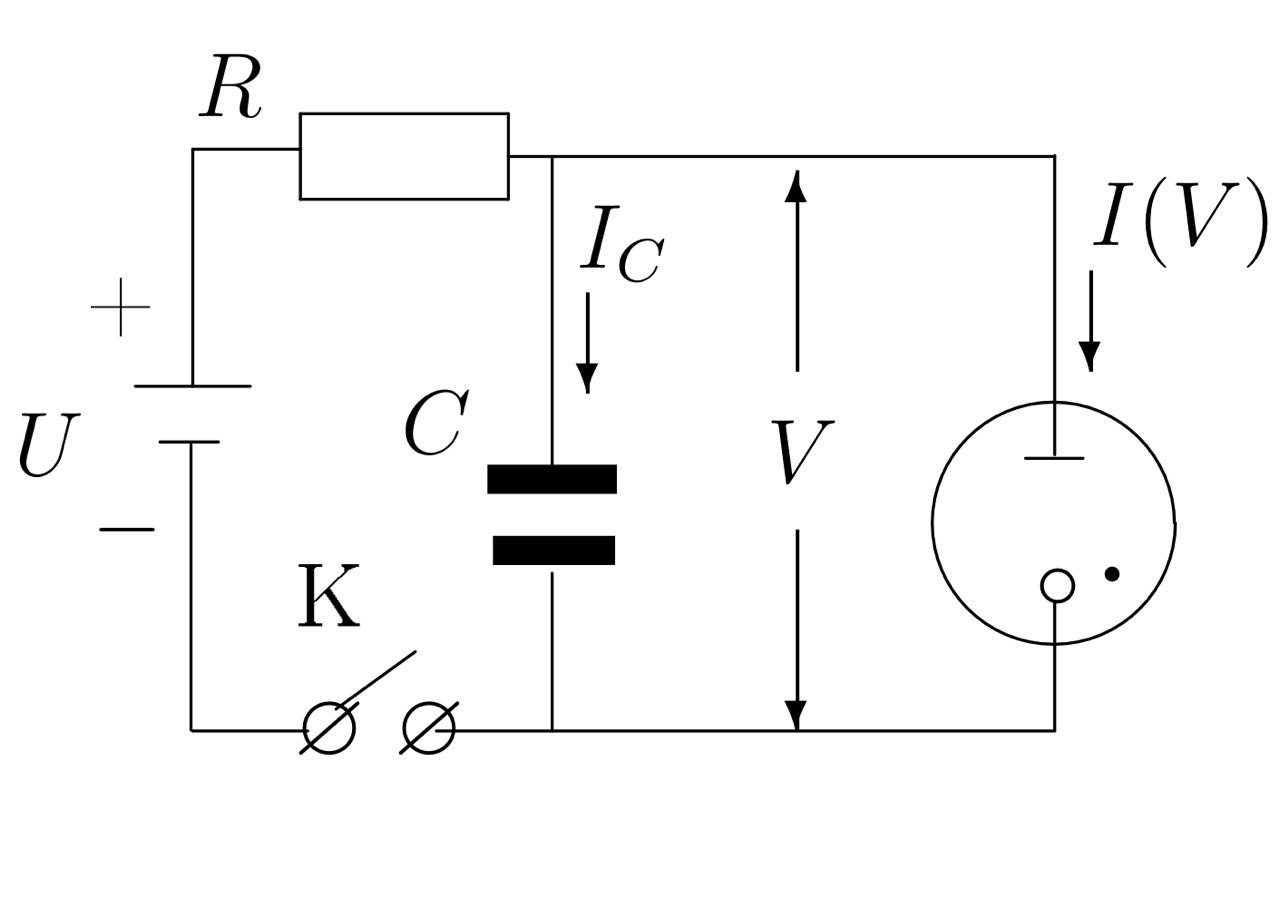
\includegraphics[width=1\textwidth]{scheme.jpg}
\caption{\centering{Принципиальная схема релаксационного генератора}}
\label{osc}
\end{center}
\end{wrapfigure}


Рассмотрим схему релаксационного генератора, представленную на рисунке слева. Пусть напряжение бата- реи $U$ больше напряжения зажигания $V_{1} .$ В обозначениях, принятых на схеме, справедливо уравнение
\begin{equation*}
I(V)=\frac{U-V}{R}
\end{equation*}
\begin{equation}
C \frac{d V}{d T}+I(V)=\frac{U-V}{R}
\end{equation}


В стационарном режиме работы, когда напряжение $V$ на конденсаторе постоянно $d V / d t=0,$ ток через лампу равен

\begin{equation}
    I_{\mathrm{cr}}=\frac{U-V}{R}
\end{equation}

\begin{wrapfigure}{r}{0.3\textwidth} 
\begin{center}
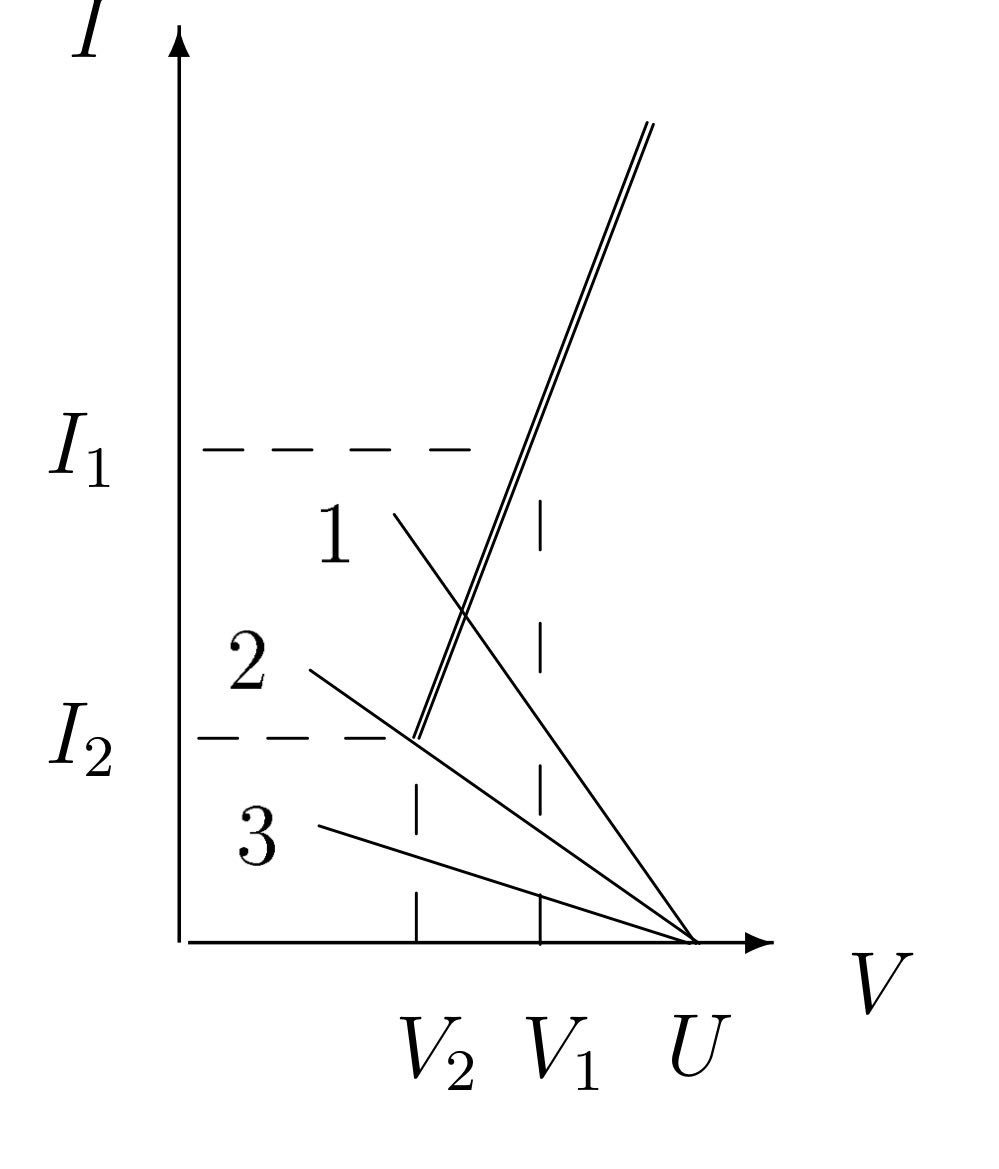
\includegraphics[width=1\textwidth]{graph2.jpg}
\caption{\centering{Режимы работы релаксационного генератора}}
\end{center}
\end{wrapfigure}

Равенство (2) может быть представлено графически (рис. 3) При разных $R$ графики имеют вид прямых, пересекаЮщихся в точке $V=U, I=0 .$ Область, где эти нагрузочные прямыие пересекают вольт-амперную характеристику лампы, соответствует стационарному режиму - при малых $R$ (прямая 1$)$ лампа горит постоянно, колебания Отсутствуют. Прямая $2,$ проходящая через точку $\left(I_{2}, V_{2}\right),$ соответствует критическому сопротивлению

\begin{equation}
R_{\mathrm{Kp}}=\frac{U-V_{2}}{I_{2}}
\end{equation}

При сопротивлении $R>R_{\text {кр }}$ нагрузочная прямая $3 \quad$ не пересекает характеристику лампы, поэтому стационарный режим невозможен. В этом случае в системе устанавливаются колебания. Рассмотрим, как происходит колебательный процесс. Пусть в начале опыта ключ К разомкнут (рис. 2) и $V=0 .$ Замкнём ключ. Конденсатор $C$ начинает заряжаться через сопротивление $R,$ напряжение на нём увеличивается (рис. 4) Как только оно достигнет напряжения зажигания $V_{1},$ лампа начинает проводить ток, причём прохождение тока сопровождается разрядкой конденсатора. В самом деле, батарея $U,$ подключённая через большое сопротивление $R,$ не может поддерживать необходимую для горения лампы величину тока. Во время горения лампы конденсатор разряжается, и когда напряжение на нём достигнет потенциала гашения, лампа перестанет проводить ток, а конденсатор вновь начнёт заряжаться. Возникают релаксационные колебания с амплитудой, равной $\left(V_{1}-V_{2}\right) .$

\begin{wrapfigure}{r}{0.3\textwidth} 
\begin{center}
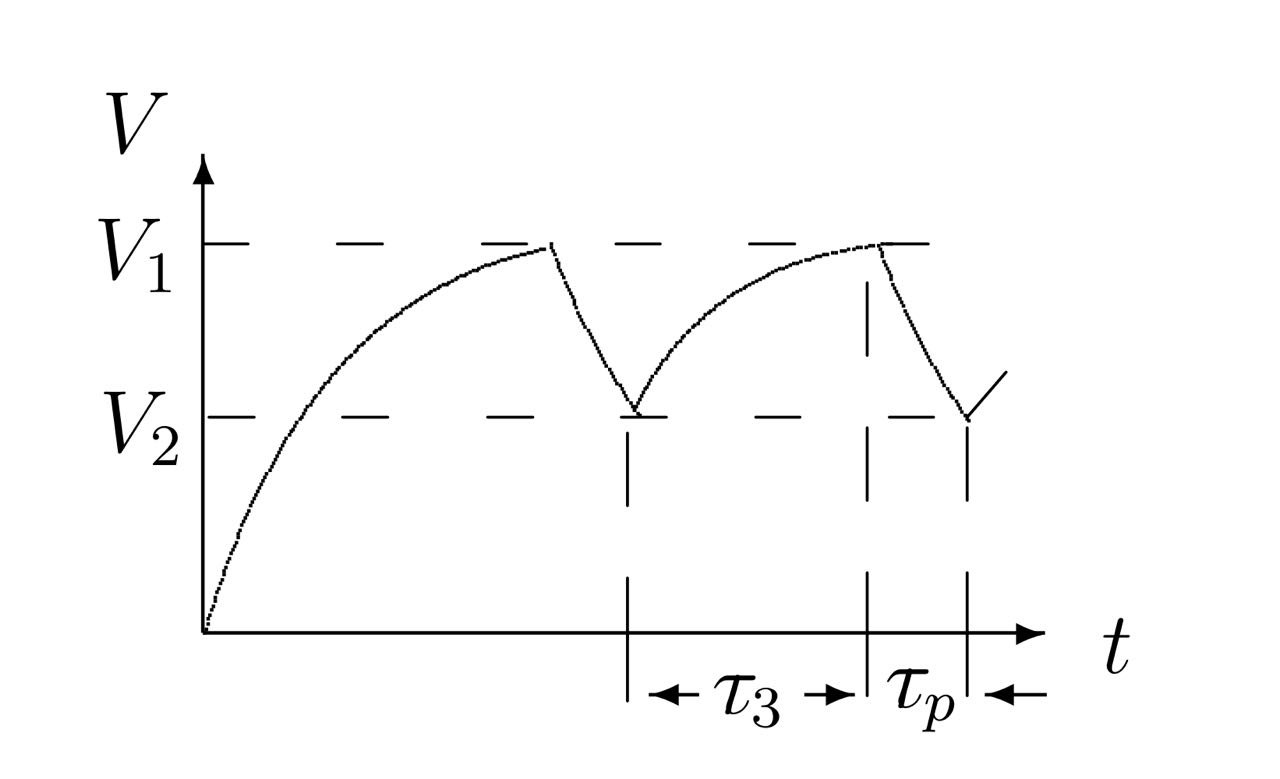
\includegraphics[width=1\textwidth]{graph3.jpg}
\caption{\centering{Осциллограмма релаксационных колебаний}}
\end{center}
\end{wrapfigure}

Рассчитаем период колебаний. Полное время одного периода колебаний Т состоит из суммы времени зарядки $\tau_{3}$ и времени разрядки $\tau_{\mathrm{p}},$ но если сопротивление $R$ существенно превосходит сопротивление Зажжённой лампы, то $\tau_{3} \gg \tau_{\mathrm{p}}$ и $T \simeq \tau_{3}($ этим случаем мы и ограничимся). Во время зарядки конденсатора лампа не горит $[I(V)=0],$ и уравнение (1) приобретает вид
\begin{equation}
R C \frac{d V}{d t}=U-V    
\end{equation}

Будем отсчитывать время с момента гашения лампы, так что $V=V_{2}$ при $t=0$ (рис. 4$) .$ Решив уравнение $(4),$ найдём
\begin{equation}
 V=U-\left(U-V_{2}\right) e^{-t /(R C)}   
\end{equation}


$\mathrm{B}$ момент зажигания $t=\tau_{3}, V=V_{1},$ поэтому
\begin{equation}
V_{1}=U-\left(U-V_{2}\right) e^{-\tau_{3} /(R C)}
\end{equation}
Из уравнений (5) и (6) нетрудно найти период колебаний:
$$
T \approx \tau_{3}=R C \ln \frac{U-V_{2}}{U-V_{1}}
$$
Развитая выше теория является приближённой. Ряд принятых при расчётах упрощающих предположений оговорен в тексте. Следует иметь в виду, что мы полностью пренебрегли паразитными емкостями и индуктивностями схемы. Не
рассматривались также процессы развития разряда и деионизация при гашении. Поэтому теория справедлива лишь в тех случаях, когда в схеме установлена достаточно большая ёмкость и когда период колебаний существенно больше времени развития разряда и времени деионизации (практически $\gg 10^{-5}$ с). Кроме того, потенциал гашения $V_{2},$ взятый из статической вольт-амперной характеристики, может отличаться от потенциала гашения лампы, работающей в динамическом режиме релаксационных колебаний.

\section{Ход работы}


\subsection{Характеристика стабилитрона}



\begin{figure}[h]
    \centering
    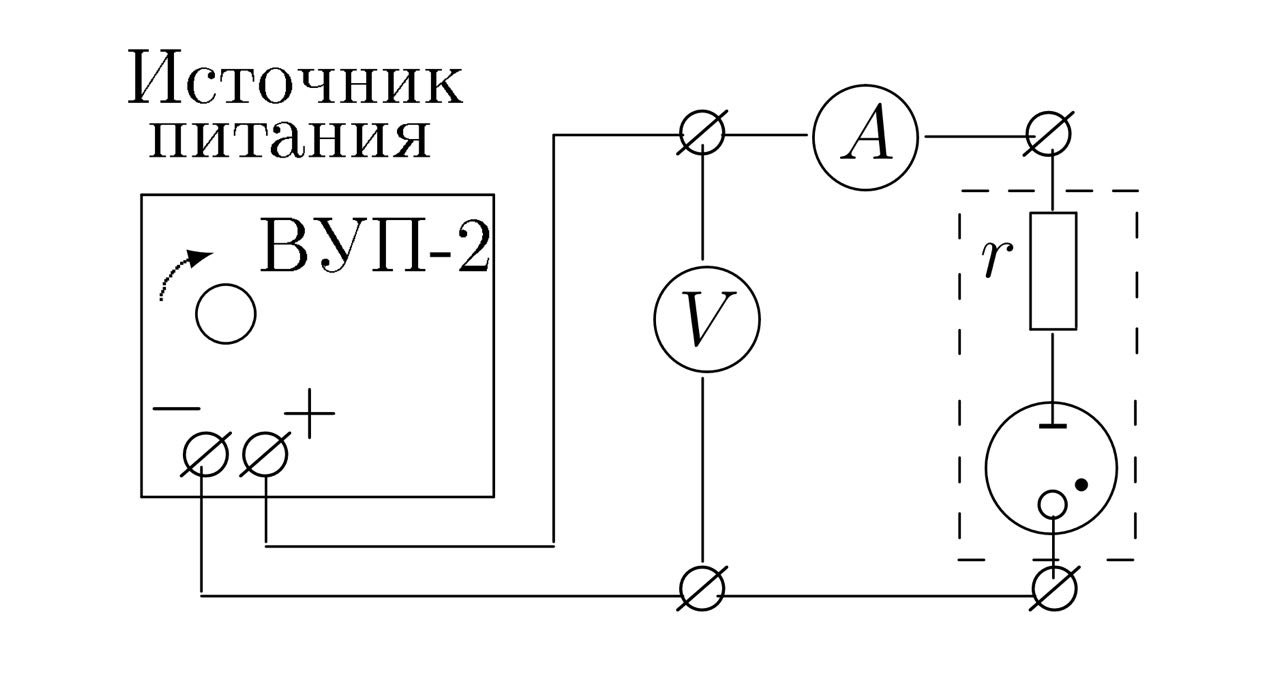
\includegraphics[scale=0.3]{scheme2.jpg}
    \label{tc}
\end{figure}








\begin{enumerate}





 \item Соберем схему, изображенную на рисунке; к выходу источника питания подключим вольтметр (мультиметр GDM), второй мультиметр используем как амперметр. Добавочное сопротивление: $r = 5,4$ кОм.

\item Включим источник в сеть и снимем вольтамперную характеристику стабилитрона с резистором $r$ при возрастании и убывании напряжения. Результаты показаний приведены в таблице 1.
\hfill \break
\hfill \break

\floatsetup[table]{capposition=top}
\begin{table}[h]
    \centering
    \begin{tabular}{|p{0.5cm}|p{2cm}|p{2cm}|p{2cm}|p{2cm}|} \hline
     \textnumero & $V$,В & $I$, мА & $\sigma_V$, В & $\sigma_I$, мА \\ \hline 
 \multicolumn{5}{|c|}{Уменьшение напряжения} \\ \hline
          1  & 89,1  & 2,89 & 0,5 & 0,05  \\ \hline
          2  & 87,7  & 2,63 & 0,5 & 0,05  \\ \hline
          3  & 84,9 & 2,14 & 0,5 & 0,05  \\ \hline
          4  & 83,2 & 1,89 & 0,5 & 0,05  \\ \hline
         \multicolumn{5}{|c|}{Увеличение напряжения} \\ \hline
      5  & 96,8 & 4,27 & 0,5 & 0,05  \\ \hline 
      6  & 99,7 & 4,77 & 0,5 & 0,05  \\ \hline 
      7  & 102,2 & 5,23 & 0,5 & 0,05  \\ \hline 
      8  & 104,2 & 5,59 & 0,5 & 0,05  \\ \hline 
    

        \end{tabular}
    \caption{Вольтамперная характеристика стабилитрона}
    \label{voltamp}
\end{table}

Полученные усреднённые значения $V1$ и $V2$:


$$V_{1} = (96,7\pm0,1) \text{ В},\quad V_{2} = (78,2\pm0,1) \text{ В}$$


\end{enumerate}

\subsection{Осциллограммы релаксационных колебаний}

\begin{enumerate}
    


\item  Соберем релаксационный генератор согласно риунку и установим на магазинах ёмкостей и сопротивлений значения $C = 50 $ нФ и $R = 900 $ кОм.

\item  Включим в сеть звуковой генератор и источник питания; установим напряжение $U \approx 118$ В; меняя частоту, получим на экране фигуру Лиссажу без самопересечений.

\item  Зафиксируем значение сопротивления $R = 250$ кОм; исследуем зависимость периода колебаний $T$ от ёмкости $C$ при постоянном напряжении источника:


\begin{figure}[H]
    \centering
    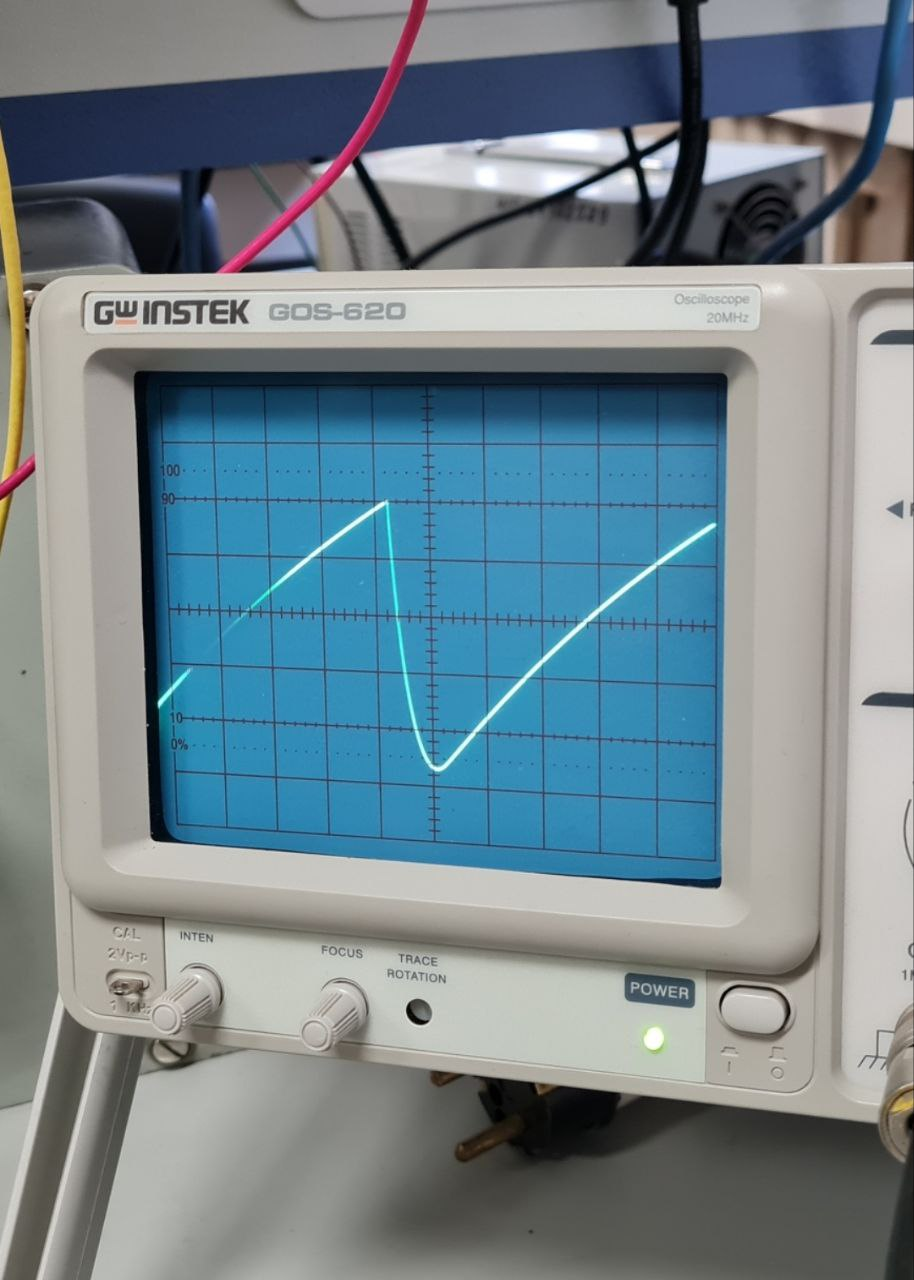
\includegraphics[scale=0.2]{pila.png}
    \caption{Пила}
    \label{tc}
\end{figure}

Заметим, что время разрядки много меньше времени зарядки : $\frac{\tau_{р}}.{\tau_{з}}\approx 0.1$


\begin{table}[H]
\centering
\begin{tabular}{|p{3cm}|p{3cm}|}
         \hline
$C$ , нФ & $T$ , мс \\ \hline\hline
50 & 9,6 \\ \hline
45 & 8,0 \\ \hline
40 & 6,4 \\ \hline
35 & 4,6 \\ \hline
32 & 3,1 \\ \hline
\end{tabular}
    \caption{Название таблицы}
\end{table}

Большее количество измерений провести не удалось, потому что в процессе возникли проблемы с изменением характеристик системы: при уменьшении ёмкости конденсатора картина на осциллографе оставалось той же. Данный факт говорит о неисправности конденсатора.

\item  Проведём серию измерений $T(C)$ при емкости 50 нФ и постоянном напряжении U, меняя величину сопротивления $R$ в пределах от максимального значения до критического $R_{кр}$ = 90 кОм


\begin{table}[h]
    \centering
    \begin{tabular}{|c|c|c|c|}
        \hline
        $R$ , кОм & $T$ , мс & $R$, кОм & $T$ , мс\\ \hline\hline
        
        900 & 36,0 & 400 & 15,5 \\ \hline
        800 & 32,0 & 300 & 11,2 \\ \hline
        700 & 28,0 & 200 & 6,2 \\ \hline
        600 & 23,5 & 100 & 6,0 \\ \hline
        500 & 20,0 & 95 & 7,5 \\ \hline
    \end{tabular}
    \caption{Завсимость $T(C)$ }
\end{table}

\end{enumerate}

\subsection{Фазовые траектории релаксационных колебаний}

Восстановим работу релакскационного генератора, установив $C = 50 $ нФ и $R = 
 = 900 $ кОм; переведем осциллограф в измерительный двухканальный режим и зафиксируем фазовую траекторию:

\begin{figure}[H]
    \centering
    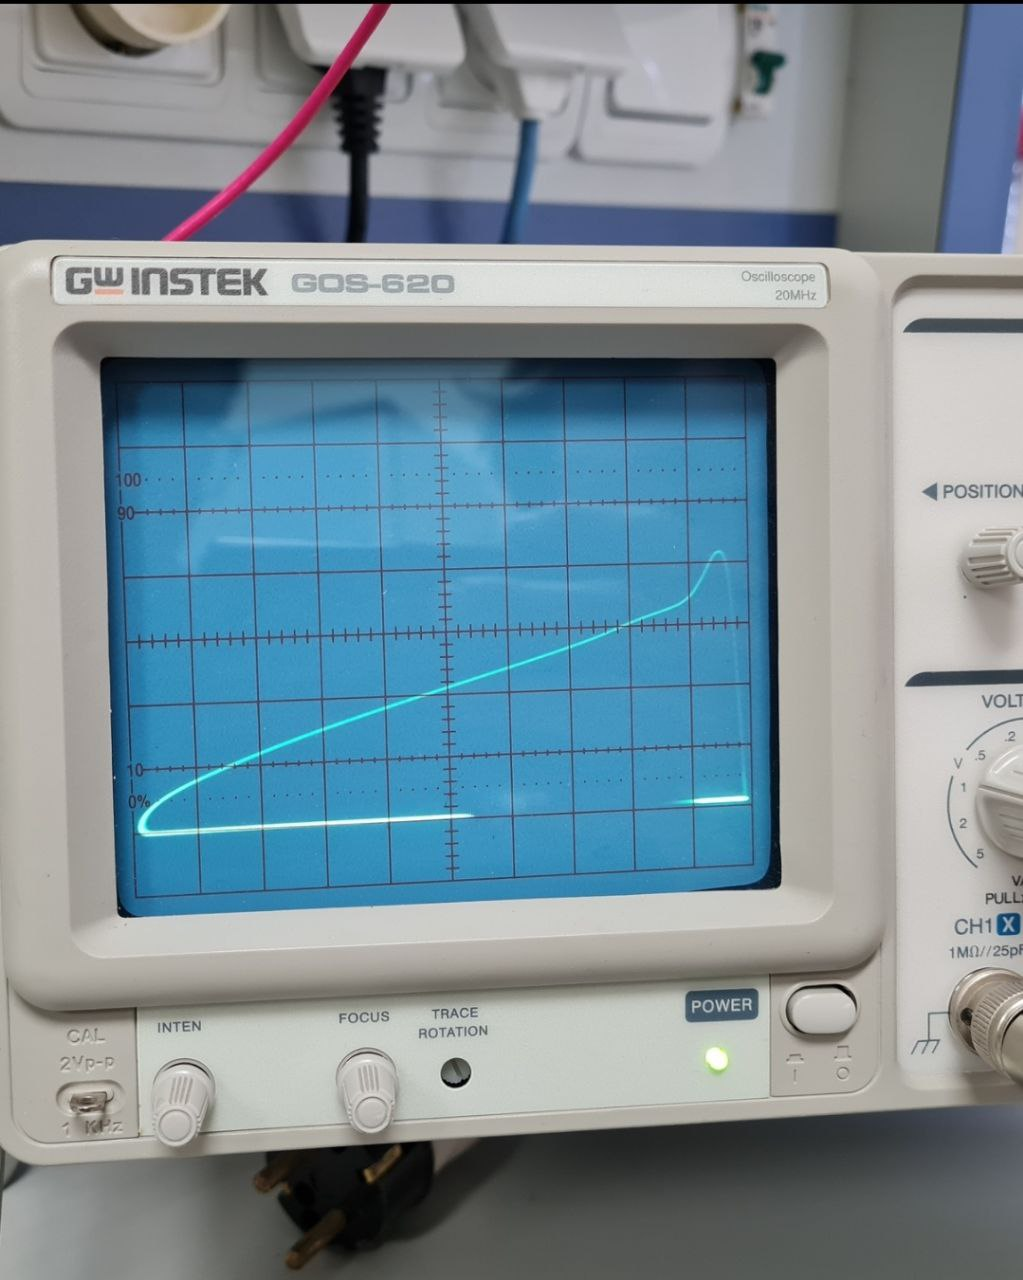
\includegraphics[scale=0.3]{fasa.png}
    \caption{Фазовая траектория}
    \label{tc}
\end{figure}


\section{Обработка результатов, сравнение с теоретическими расчетами}

\begin{enumerate}
   


 \item  Построим графики зависимости $I(U)$ для системы, состоящей из стабилитрона и сопротивления $r$, и для стабилитрона с вычетом падения напряжения $r$:

\begin{figure}[h]
    \centering
    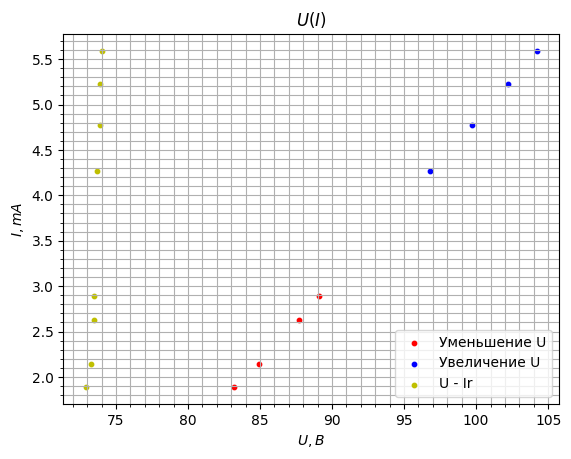
\includegraphics[scale=0.65]{F(x).png}
    \caption{Зависимость I(U)}
    \label{tc}
\end{figure}

 \item  Сравним теоретическую и эксперементальную зависимости $T(C)$ и $T(R)$, проиллюстрировав их на графиках:

\begin{figure}[H]
    \centering
    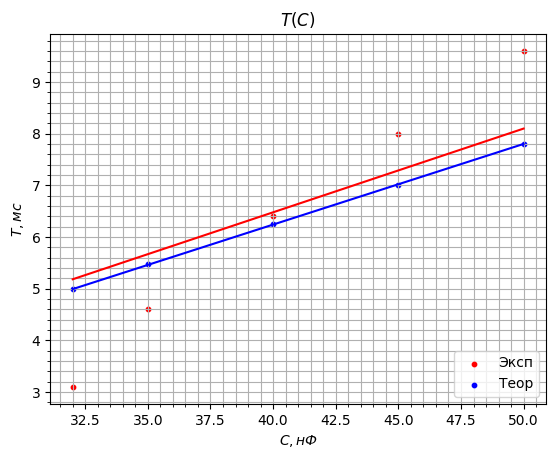
\includegraphics[scale=0.7]{tttt.png}
    \caption{Зависимость периода колебаний от ёмкости}
    \label{tc}
\end{figure}

\begin{figure}[H]
    \centering
    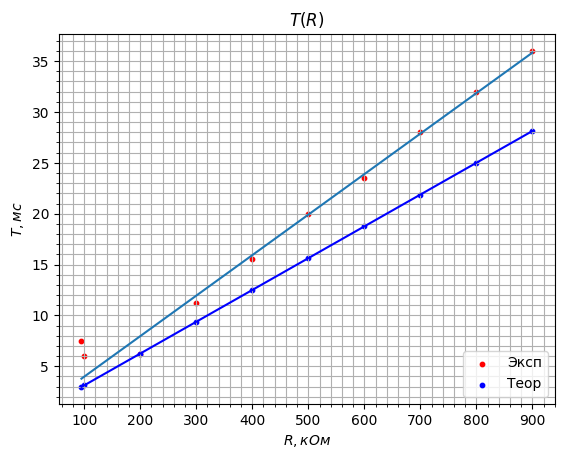
\includegraphics[scale=0.7]{G22.png}
    \caption{Зависимость периода колебаний от сопротивления }
    \label{tc}
\end{figure}

Видно, что в обоих опытах последние экспериментальные точки сильно отдалены от аппроксимированных прямых. Такое отклонение можно объяснить неисправностью нашего конденсатора: при понижении ёмкости ниже 35 нФ показания приборов либо изменялись, либо оставались почти постоянными. 

Также нетрудно заметить, что теоретические и экспериментальные результаты различаются несильно. Из формулы (6) следует:

\begin{equation}
V_{2}=U-\left(U-V_{1}\right) e^{k},
\end{equation}

где k - коэффициент наклона прямой. Пр постоянном сопротивлении $k = R \ln \frac{U-V_{2}}{U-V_{1}}$, при постоянной ёмкости конденсатора $k = C \ln \frac{U-V_{2}}{U-V_{1}}$. Отсюда находим

\begin{equation}
V_{2R} = (77\pm1)\text{ В} , V_{2C} = (74\pm1)\text{ В}
\end{equation}


Теоретические значения $V2$:

\begin{equation}
V_{2R} = (76\pm1)\text{ В}, V_{2C} = (73\pm1)\text{ В}
\end{equation}


\end{enumerate}

\section{Вывод и обсуждение результатов}

\begin{enumerate}
    \item Как видно, вольт-амперная характеристика нормального тлеющего заряда близка к упрощенной (ср. рис.3 и рис.7). Также видно, что при вычтенном падении напряжения на дополнительном сопротивлении $r$ график $I(U)$ может быть очень хорошо приближен вертикальной прямой. Cтоит отметить, что нами было снято малое число точек, а потому реальная вольт-амперная характеристика может быть отлична от приведённой. В этом состоит минус организации эксперимента.
    \item Экспериментальные зависимости $T(C)$ и $T(R)$ относительно хорошо приближаются прямыми. Это значит, что наша теоретическая модель описания релаксационных колебаний работает. Кроме того, теоретические и экспериментальные данные почти не отличаюся. Особенно хорошо это выражено на графике зависимости $T(C)$. Такое расхождение можно объяснить главным образом неисправностью конденсатора (см. выше) и возможным сложным поведением плазмы при протекании тока через газонаполненный диод. Этим же объясняется расхождение в расчёте потенциала гашения.
\end{enumerate}



\end{document}
